\section{Mechanism of On-Policy Distillation}

\subsection{Why Does OPD Sometimes Fail?}

\paragraph{Student Prefixes Distort the Teacher State.}
A central challenge in OPD is that the teacher is conditioned on
student-generated prefixes rather than its own trajectory. Although a strong
teacher may solve the problem independently, a partial student trajectory can
force it into an intermediate reasoning state that it would not have reached
on its own. To quantify this effect, we conduct a prefix-conditioned teacher
evaluation on GPQA-Diamond, using Qwen3-1.7B as the student and Qwen3-14B as
the teacher. The standalone teacher achieves $\textbf{62.1\%}$ accuracy, whereas
the student-prefix-conditioned teacher drops to $\textbf{46.0\%}$ accuracy
(details in Appendix~\ref{app:actionspace}). Thus, OPD supervision can become
weaker than the teacher's standalone capability if the teacher continues from student prefixes. Figure~\ref{fig:semantic_conflict_example} illustrates this failure mode at the
token level. Given a student prefix that has already committed to one reasoning
branch, the teacher assigns high probability to tokens such as ``wait'' and
``but,'' which revise or redirect the trajectory rather than extend it. This
creates a local semantic conflict between the student's current path and the
teacher's preferred path. In math reasoning, such unreliable supervision encourages verbose and inconsistent
reasoning.

\begin{figure}[t]
    \centering
    \begin{minipage}[t]{0.5\textwidth}
        \vspace{0pt}
        \centering
        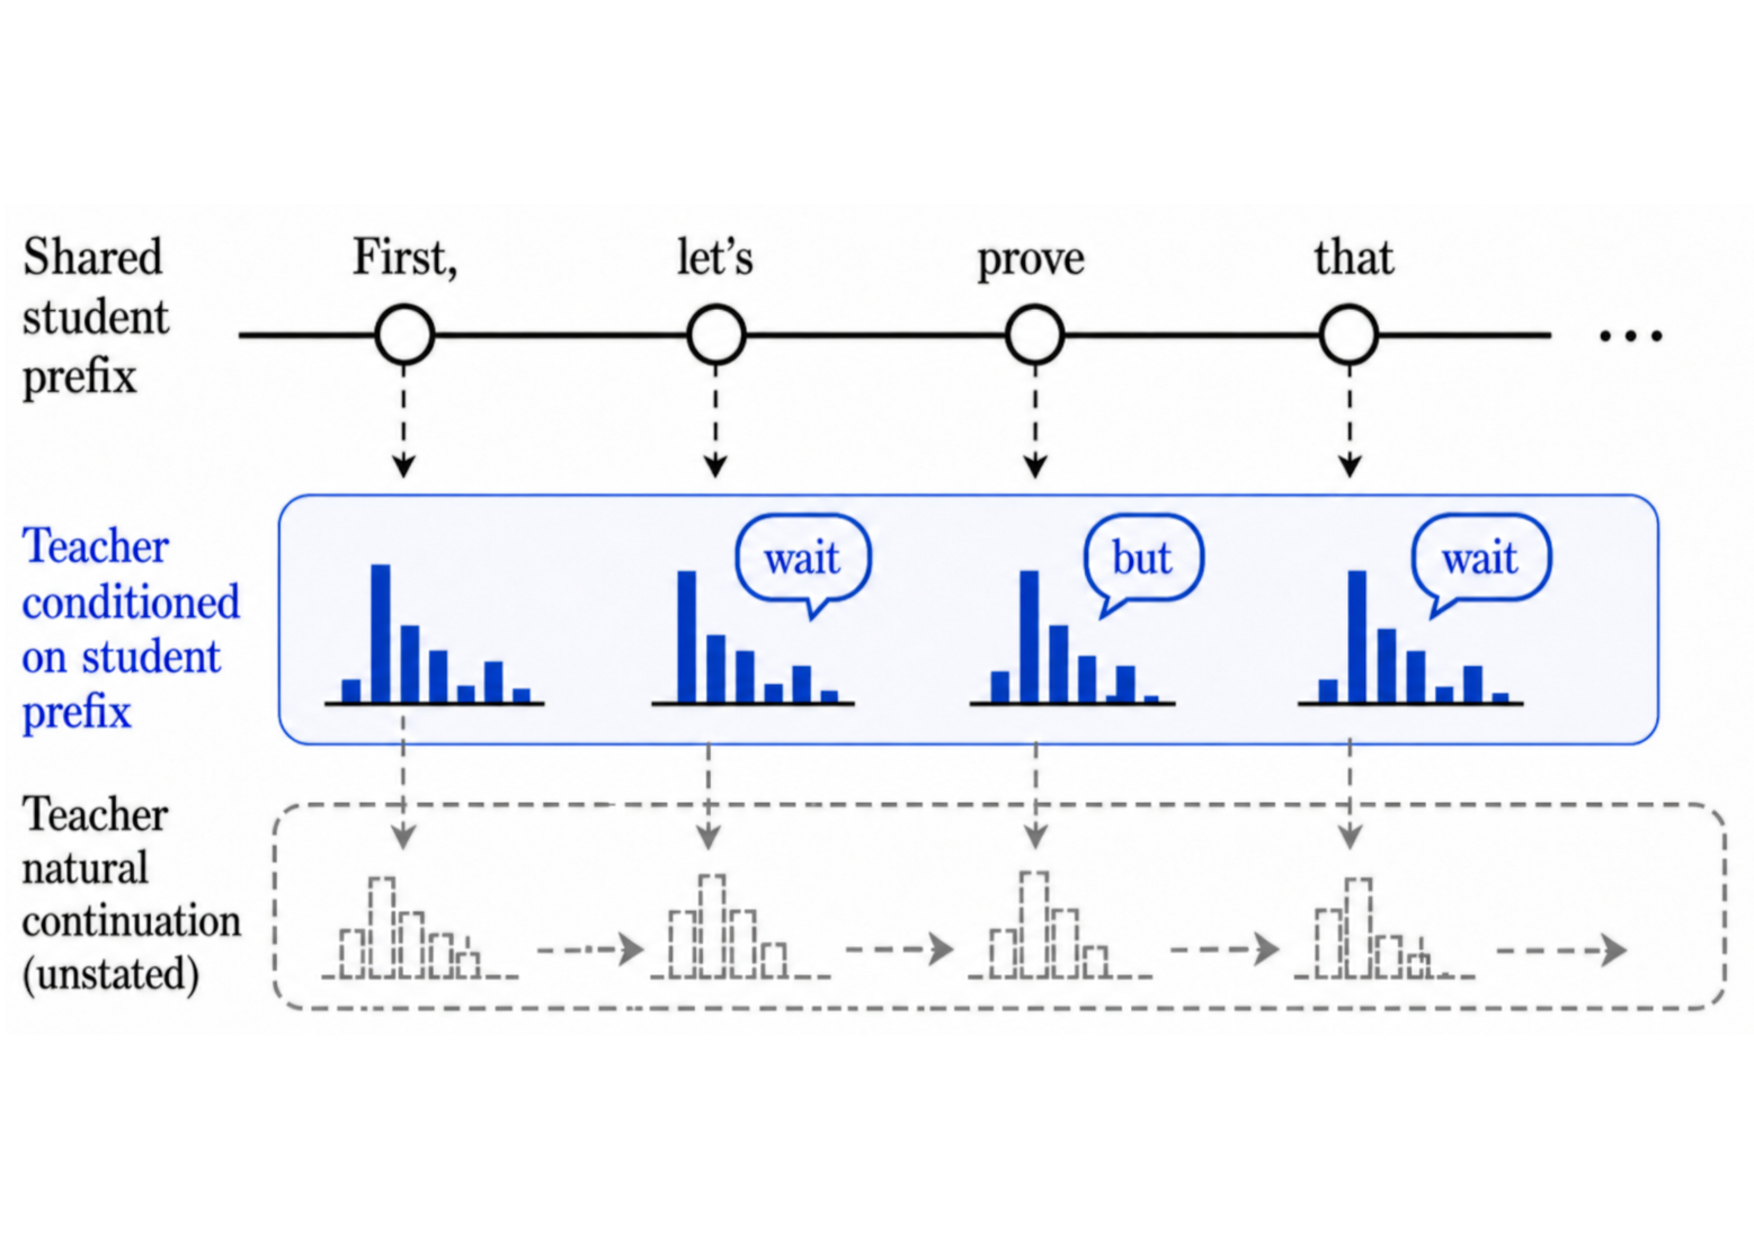
\includegraphics[width=\textwidth]{figures/opdfail.pdf}
    \end{minipage}
    \begin{minipage}[t]{0.45\textwidth}
        \vspace{0pt}
        \caption{Local semantic conflict in OPD. If the teacher's preferred
        path is inconsistent with the student prefix, teacher may encourage branch switching rather than branch refinement. This often
        appears as high probability assigned to revision tokens such as
        \textbf{``wait''} and \textbf{``but''}, which attempt to redirect the
        trajectory.}
        \label{fig:semantic_conflict_example}
    \end{minipage}
\end{figure}




\paragraph{The pitfall of unnormalized TopK Reverse KL.}
\label{curse_topk}

To reduce the GPU memory peak of reverse-KL distillation, we usually use the teacher's or the student's TopK set to compute a surrogate OPD loss. However, this may change the optimization stability and lead to model collapse in Figure \ref{fig:3opdcollapse}. Consider the full-vocabulary reverse KL in Equation \ref{eq:fullreverseKL}. A TopK truncation keeps only a subset $S_K(y_{<t})\subset\mathcal V$:
\begin{equation}
\mathcal L_{\mathrm{Top}\text{-}K\text{-}\mathrm{RKL}}(t)
=
\sum_{v\in S_K(y_{<t})}
\pi_S(v\mid x, y_{<t})\log\frac{\pi_S(v\mid x,y_{<t})}{\pi_T(v\mid x,y_{<t},I)}.
\label{eq:topkrevKL}
\end{equation}

The difference is in the gradient. For the full-vocabulary objective in Equation \ref{eq:fullreverseKL},
the constant term \textbf{+1} can be removed because
\begin{equation}
\sum_v p_\theta(v)\nabla_\theta\log p_\theta(v)  = 0
\end{equation}
However, this no longer holds for TopK:
\begin{equation}   
\sum_{v\in S_K(y_{<t})}\pi_S(v\mid x,y_{<t})\nabla_\theta \log \pi_S(v\mid x,y_{<t})
=
\nabla_\theta \sum_{v\in S_K(y_{<t})}\pi_S(v\mid x,y_{<t})
\neq 0.
\end{equation}
The \textbf{+1} term in the gradient remains:
\begin{equation} 
\nabla_\theta \mathcal L_{\mathrm{Top}\text{-}K\text{-}\mathrm{RKL}}(t)
=
\sum_{v\in S_K(y_{<t})}
\pi_S(v\mid x,y_{<t})
\left(
\log\frac{\pi_S(v\mid x,y_{<t})}{\pi_T(v\mid x,y_{<t},I)}\textbf{+1}
\right)
\nabla_\theta \log \pi_S(v\mid x,y_{<t}),
\end{equation}


Thus TopK truncation changes the update rule: a token is promoted only if
$
\pi_T(v \mid x,y_{<t},I) > e\,\pi_S(v \mid x,y_{<t}).
$
Teacher-preferred tokens with smaller teacher-student margins are still suppressed, biasing the student away from the teacher distribution and potentially toward unstable low-probability continuations.




\subsection{OPSD Learns a PI-Free Policy.}

\begin{figure}[t]
    \centering
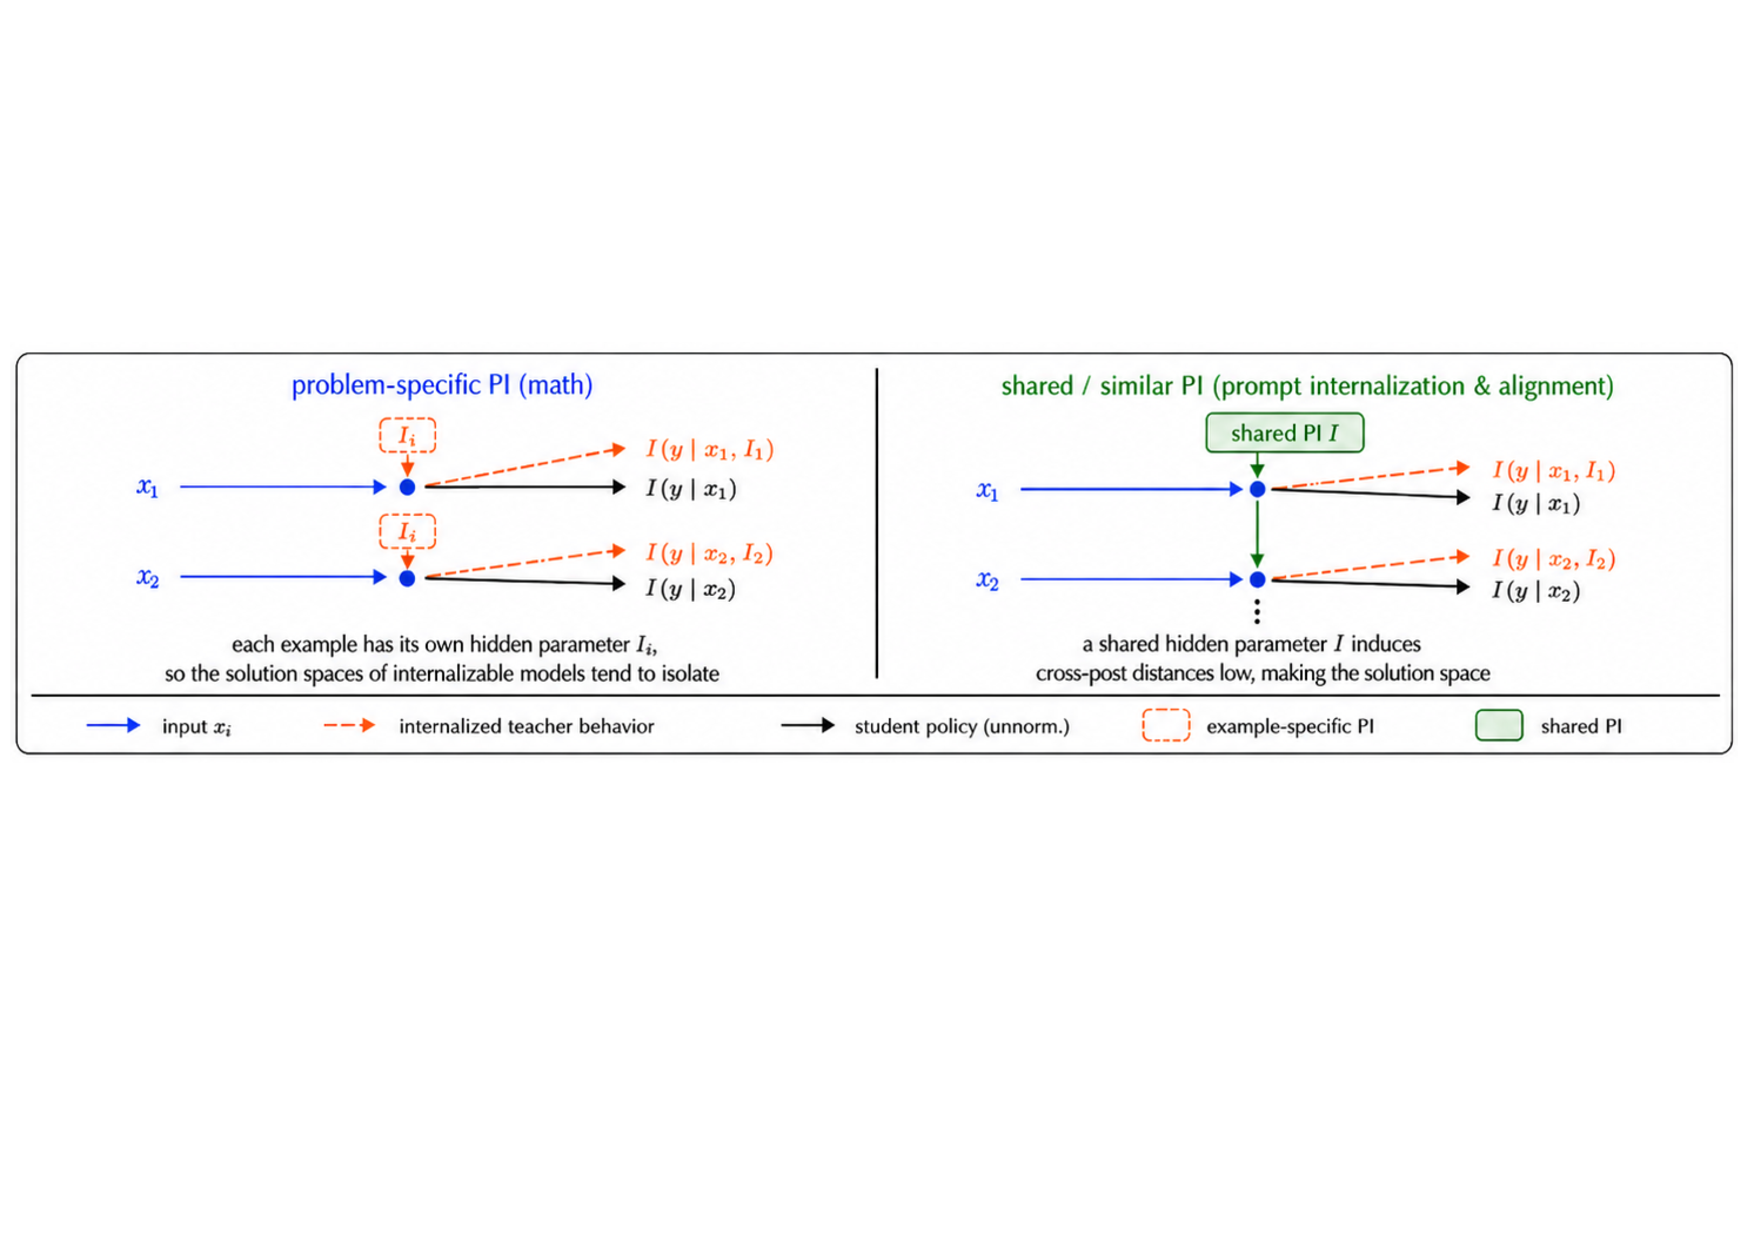
\includegraphics[width=0.75\textwidth]{figures/OPSD_diffPI.pdf}
    % \vspace{-2mm}  % 根据需要调整，移除子图后可能不需要
    \caption{
    Effectiveness of OPSD depends on the structure of privileged information I.
    }
    \label{fig:8opsd}
\end{figure}



\begin{figure*}[t]
    \centering
    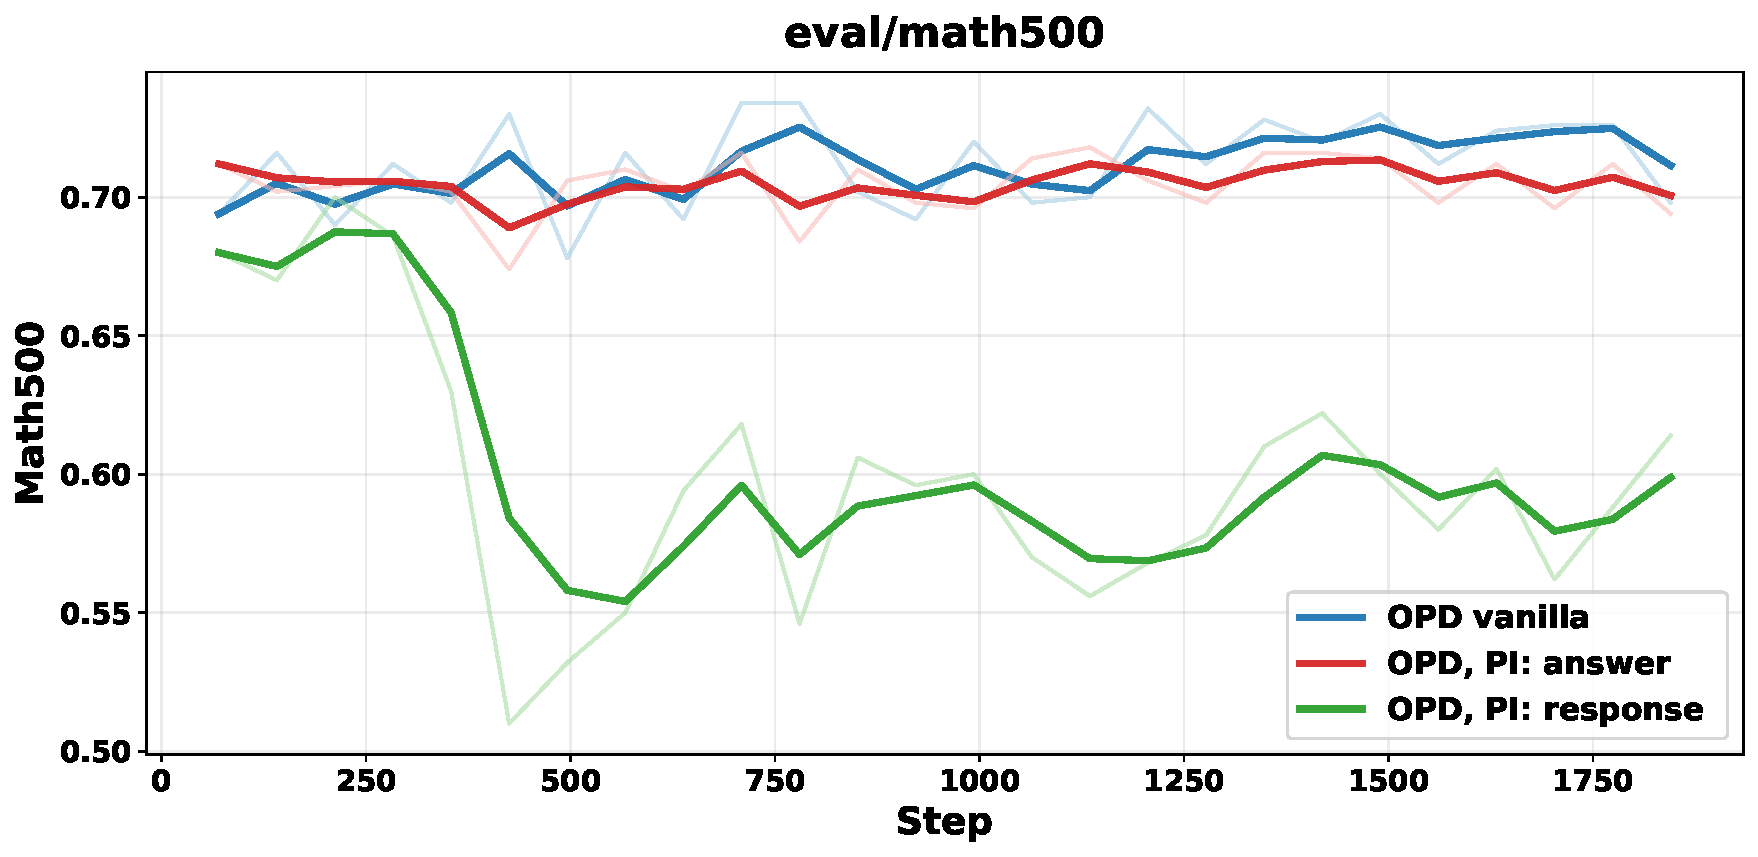
\includegraphics[width=0.33\textwidth]{figures/math500_opdPI.pdf}
    \hfill
    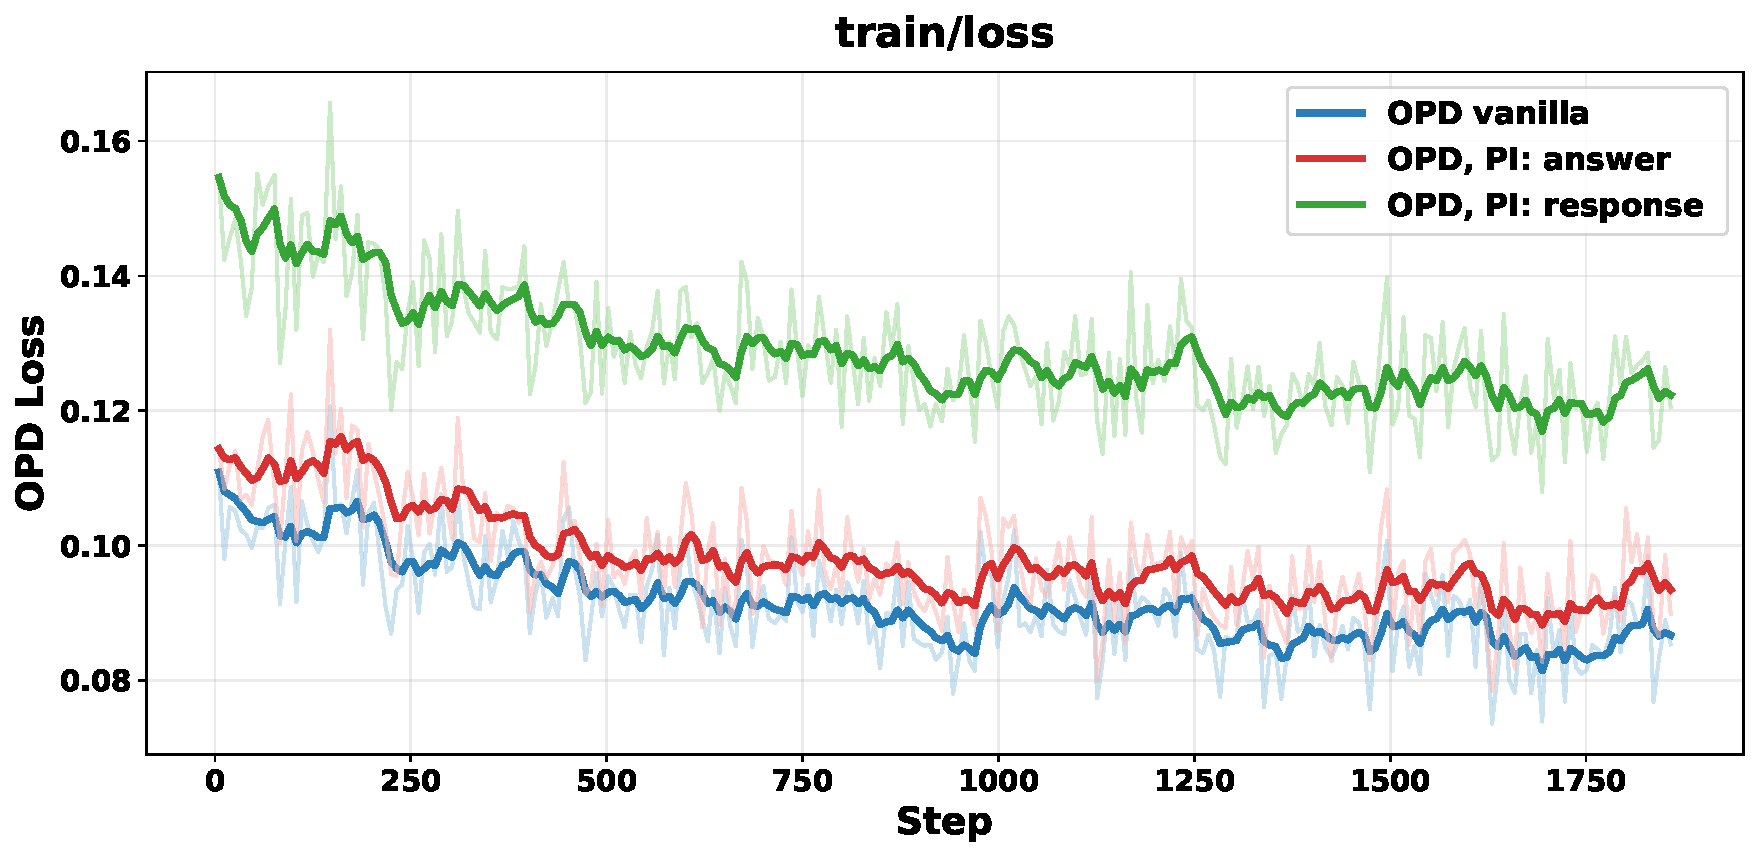
\includegraphics[width=0.33\textwidth]{figures/loss_opdPI.pdf}
    \hfill
    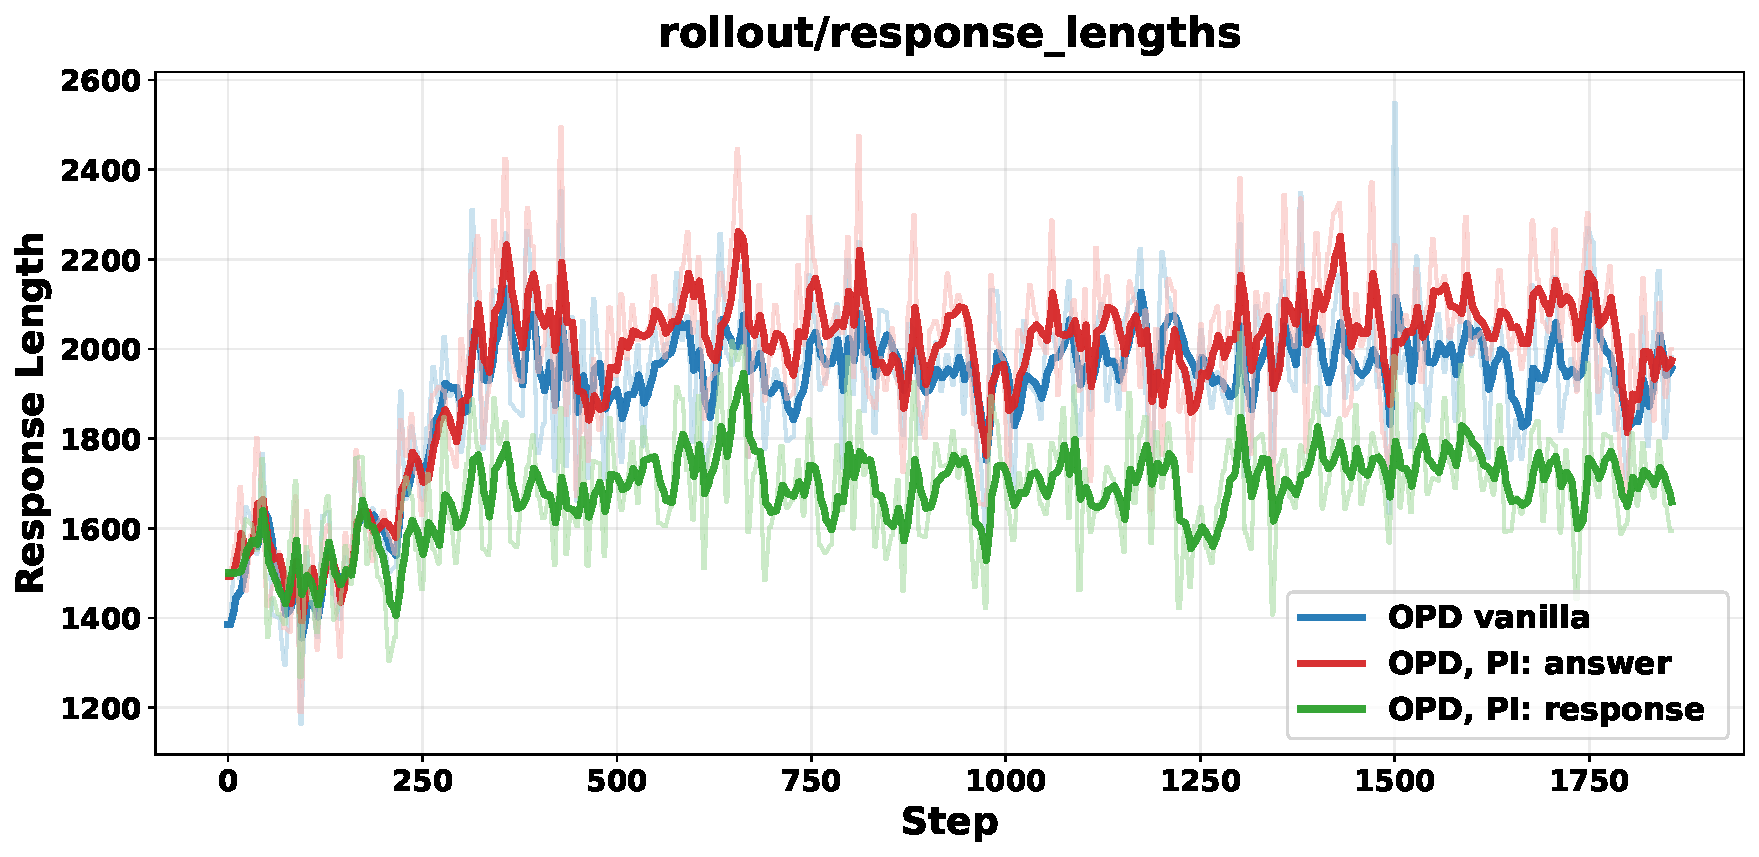
\includegraphics[width=0.32\textwidth]{figures/length_opdPI.pdf}

\caption{
\textbf{PI does not improve OPD on math reasoning with a stronger teacher.}
Using a Qwen3-8B teacher and a Qwen3-1.7B student on OpenThoughts, both final-answer PI and full-response PI underperform vanilla OPD.
PI-conditioned OPD leads to higher KL loss.
}
    \label{fig:9OPDPI}
\end{figure*}




Let $x$ denote the question and $I$ denote the privileged information (PI).
Since the student does not observe $I$, OPSD optimizes
\begin{equation}
\min_{p_S}\;
\mathbb{E}_{(x,I)\sim\mathcal D}
\Big[
D_{\mathrm{KL}}\!\big(p_S(\cdot\mid x)\,\|\,p_T(\cdot\mid x,I)\big)
\Big].
\end{equation}
The optimal student is the normalized geometric mean of the PI-conditioned teacher distributions:
\begin{equation}
p_S^\star(y\mid x)
=
\frac{
\exp\left(
\mathbb{E}_{I\sim\mathcal D(\cdot\mid x)}
\log p_T(y\mid x,I)
\right)
}{
\sum_{y'}
\exp\left(
\mathbb{E}_{I\sim\mathcal D(\cdot\mid x)}
\log p_T(y'\mid x,I)
\right)
}.
\end{equation}
This form indicates that OPSD can distill behavior that is consistently
supported under different PI. Outputs that receive high probability under
some PI but low probability under others are suppressed. Figure~\ref{fig:8opsd} illustrates why the structure of PI ($I$) matters.
When PI is problem-specific, as in math reasoning, different examples depend
on different PI $I_1,I_2,I_3$. These parameters can
induce incompatible teacher behaviors, so the student is driven toward the common pattern of these incompatible teacher policies. This makes the student substantially weaker than the PI-conditioned teacher. In contrast, when
PI follows a similar latent structure, as in prompt internalization or
alignment, many examples are governed by the same underlying rule $I$. The
student can then compress the teacher's PI-conditioned behavior into a reusable
inductive bias.



To test whether math PI provides useful supervision, and to rule out limited
teacher capability as the cause of OPSD failure, we use a stronger Qwen3-8B
teacher to train a Qwen3-1.7B student with vanilla OPD, answer-PI OPD, and
response-PI OPD. As shown in Figure~\ref{fig:9OPDPI}, PI remains \textbf{unhelpful}:
both PI-conditioned methods underperform vanilla OPD, with response-PI
performing worst. Their distillation losses (at step 0) follow
\emph{OPD, PI: response} $>$ \emph{OPD, PI: answer} $>$ \emph{OPD vanilla},
suggesting that PI increases teacher-student mismatch. The higher loss of response-PI indicates that a longer PI induces a larger distributional
shift rather than a better distillation signal.


\section{Solutions}

\subsection{Designing an appropriate OPD loss.}


\begin{figure}[t]
    \centering
    \begin{subfigure}[t]{0.32\textwidth}
        \centering
        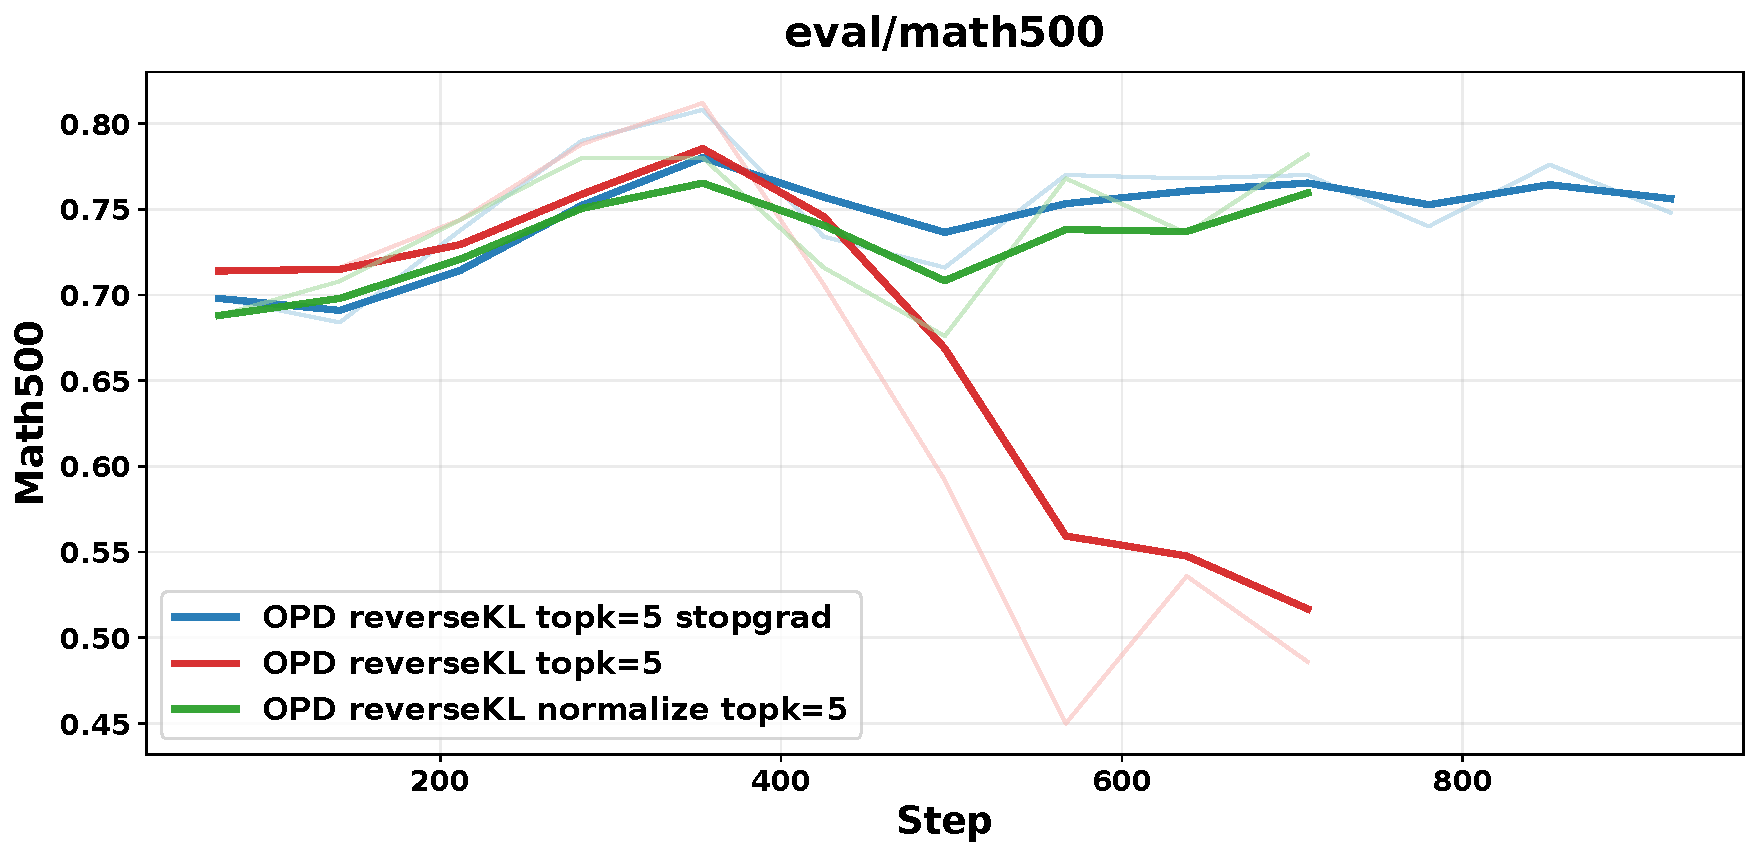
\includegraphics[width=\textwidth]{figures/top5_eval_math500.pdf}
        \label{fig:4b_char}
    \end{subfigure}
    \hfill
    \begin{subfigure}[t]{0.33\textwidth}
        \centering
        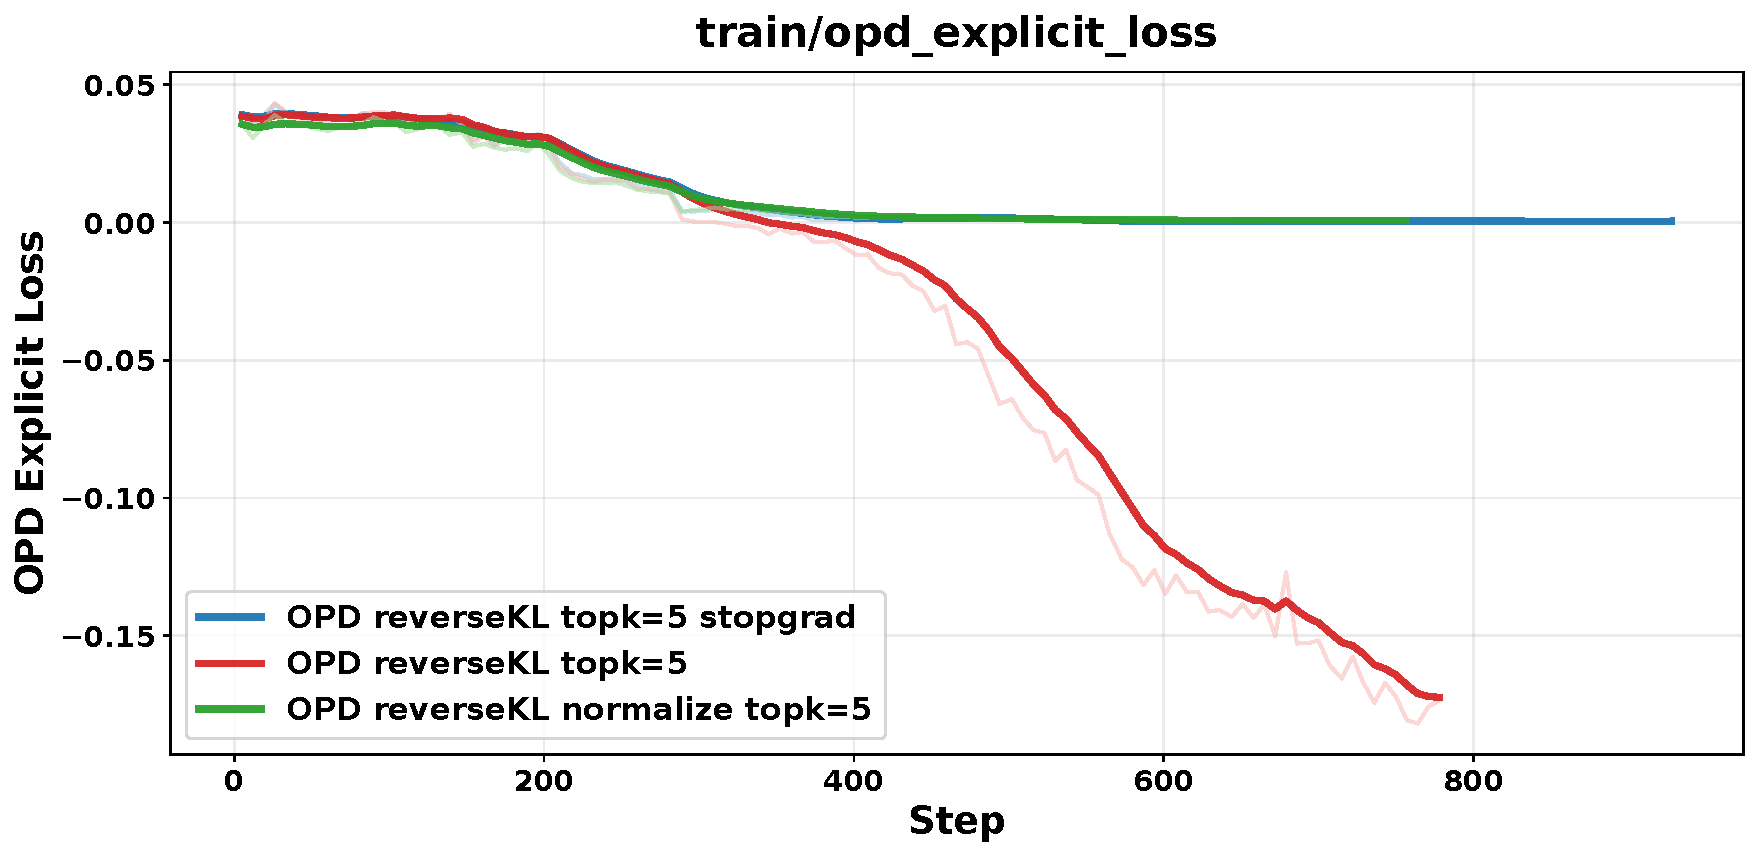
\includegraphics[width=\textwidth]{figures/top5_opd_explicit_loss.pdf}
        \label{fig:4b_emo}
    \end{subfigure}
    % \vspace{0.5em}
    \hfill
    \begin{subfigure}[t]{0.33\textwidth}
        \centering
        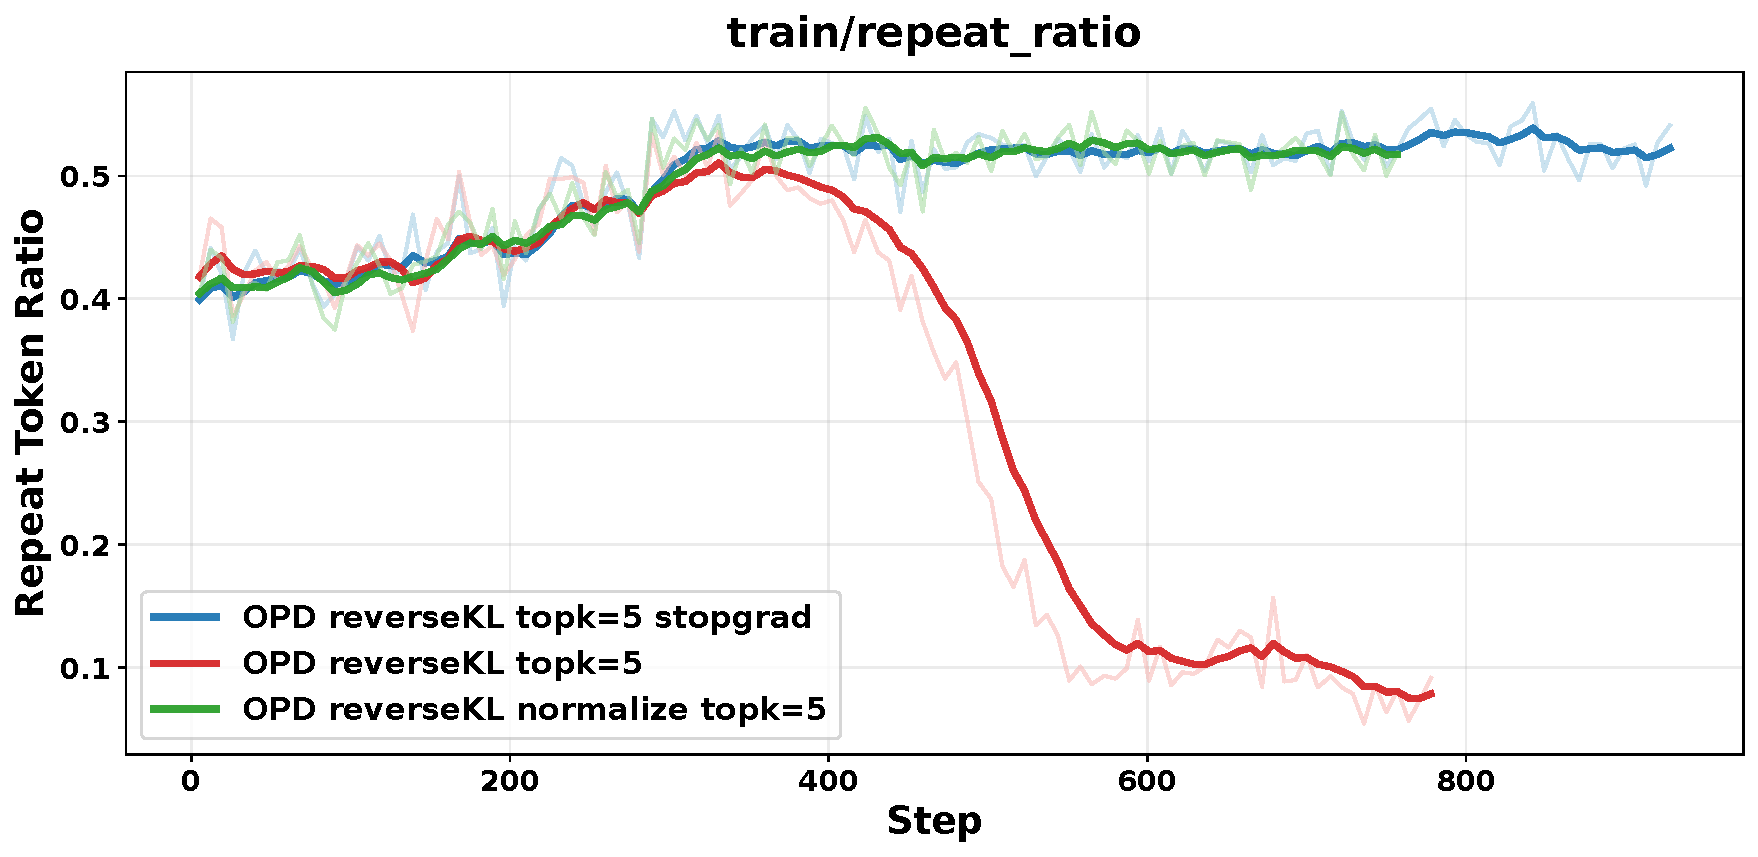
\includegraphics[width=\textwidth]{figures/top5_repeat_ratio.pdf}
        \label{fig:8b_char}
    \end{subfigure}
    \hfill
    % \begin{subfigure}[t]{0.33\textwidth}
    %     \centering
    %     \includegraphics[width=\textwidth]{figures/top5_task_reward_mean.pdf}
    %     \label{fig:8b_emo}
    % \end{subfigure}
    
    \begin{subfigure}[t]{0.32\textwidth}
        \centering
        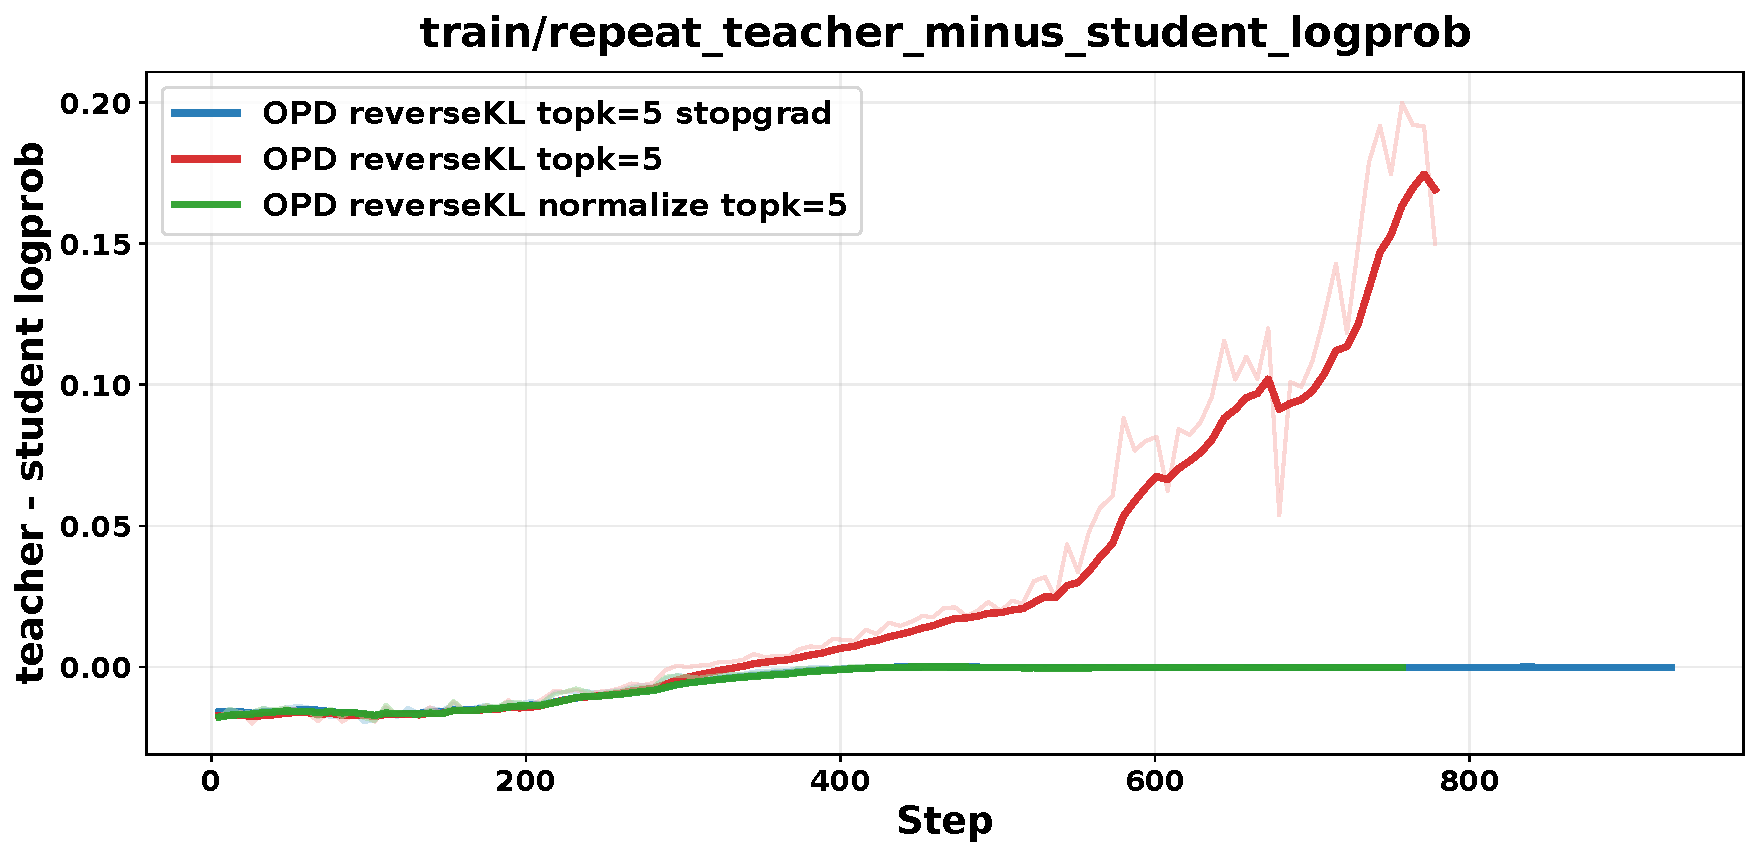
\includegraphics[width=\textwidth]{figures/top5_teacherstudent_repeat_logprob.pdf}
        \label{fig:4b_char}
    \end{subfigure}
    \hfill
    \begin{subfigure}[t]{0.33\textwidth}
        \centering
        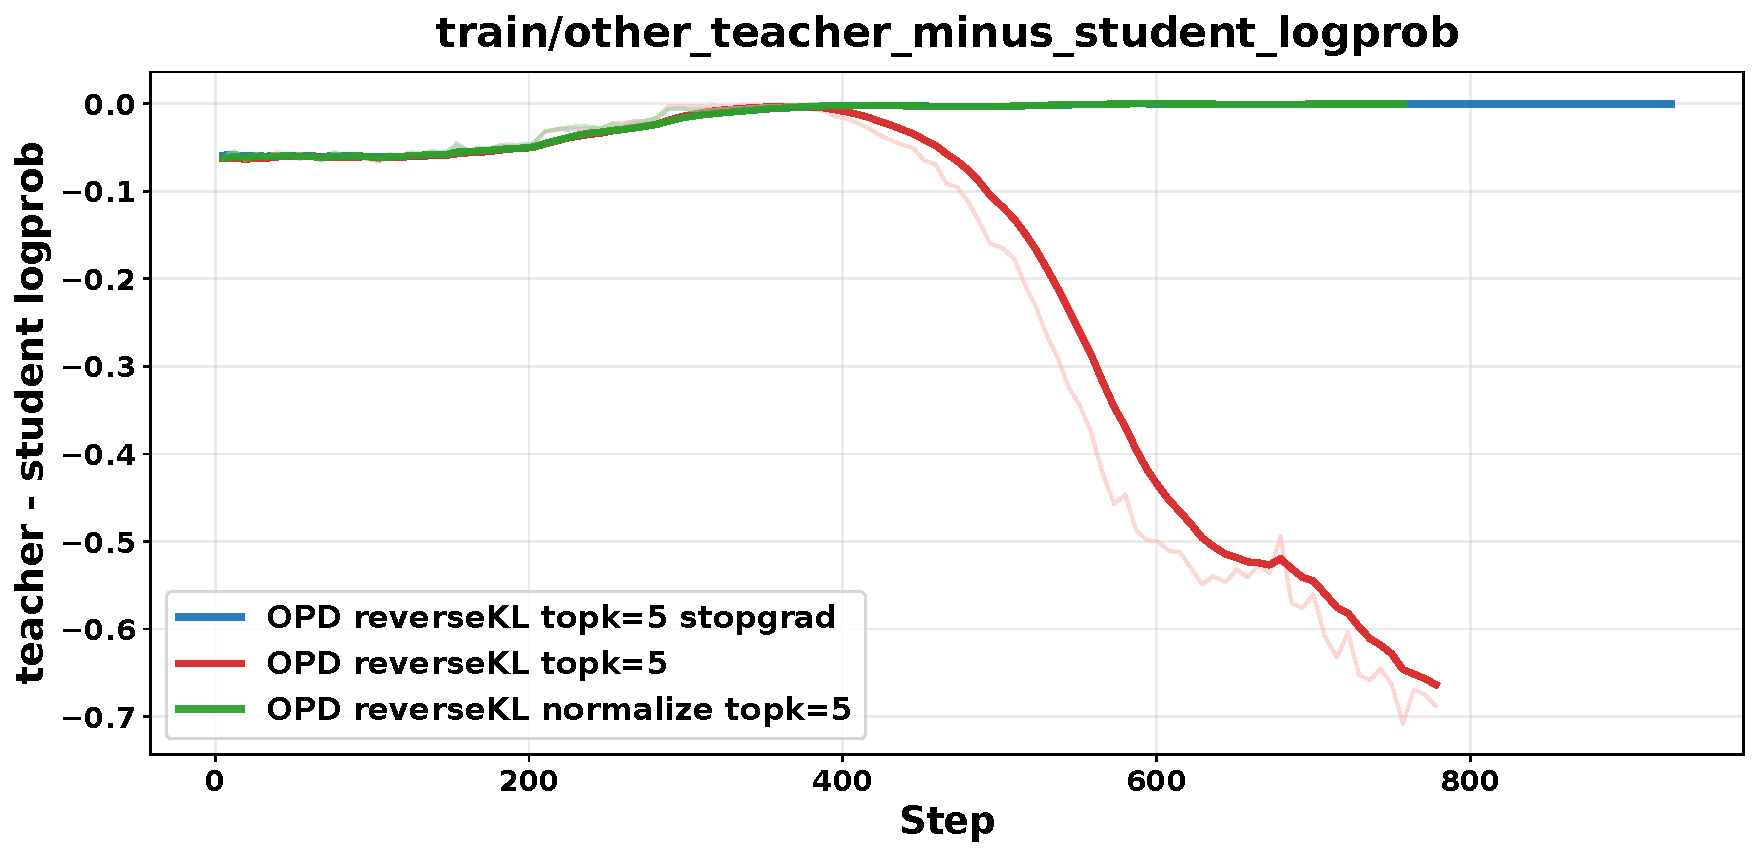
\includegraphics[width=\textwidth]{figures/top5_teacherstudent_other_logprob.pdf}
        \label{fig:4b_emo}
    \end{subfigure}
    % \begin{subfigure}[t]{0.24\textwidth}
    %     \centering
    %     \includegraphics[width=\textwidth]{figures/top5_student_logprob.pdf}
    %     \label{fig:8b_char}
    % \end{subfigure}
    \hfill
    \begin{subfigure}[t]{0.33\textwidth}
        \centering
        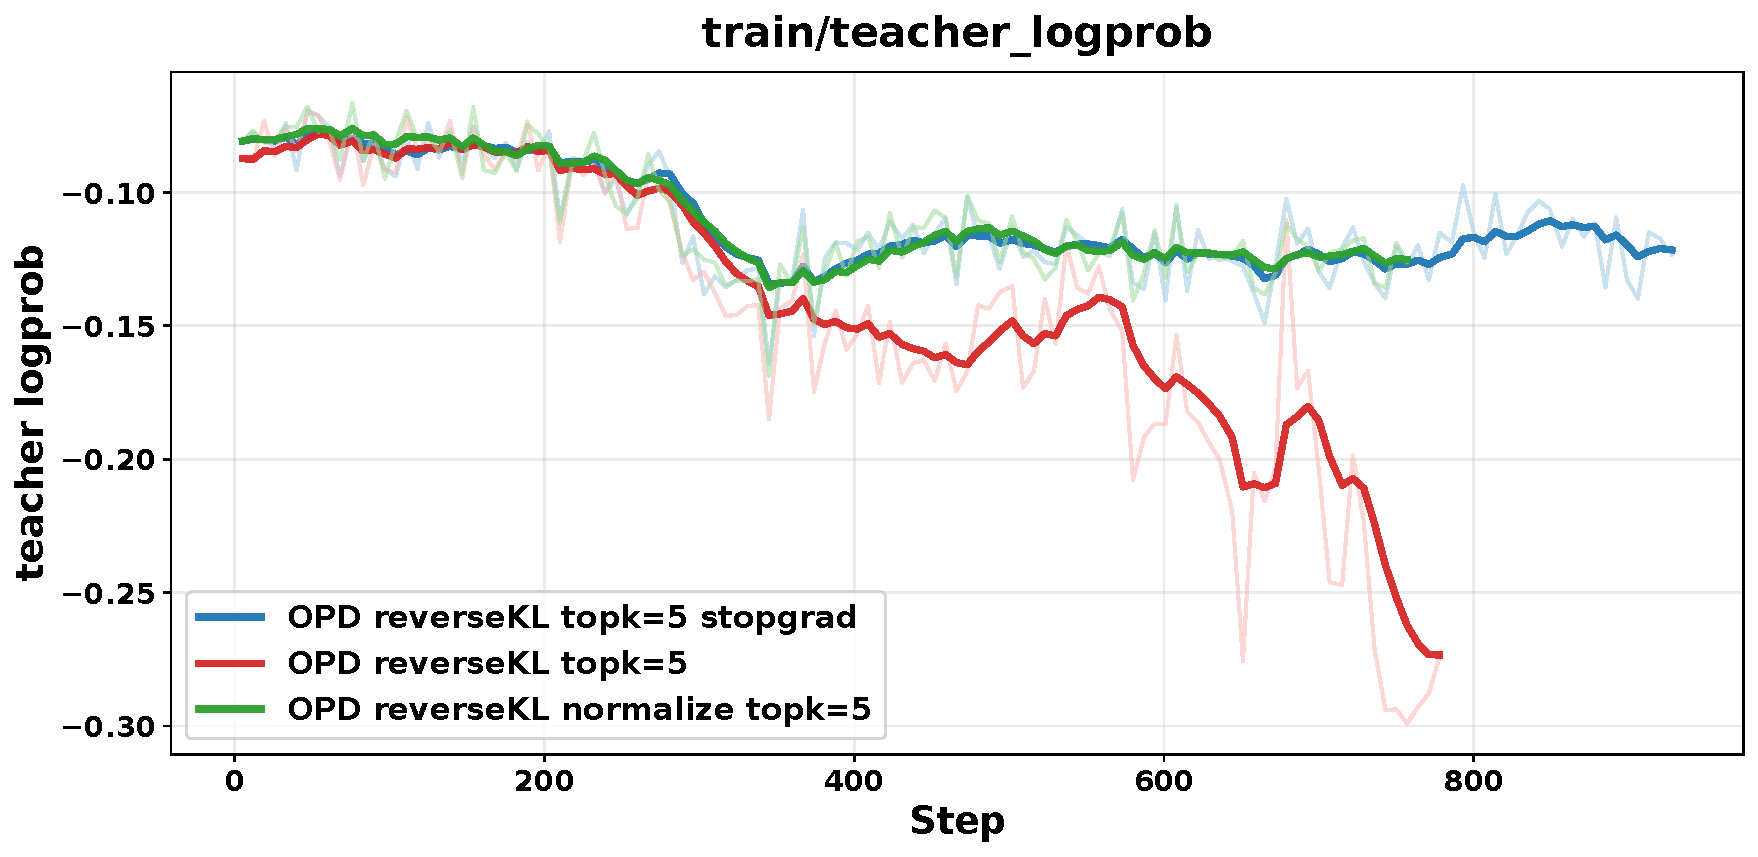
\includegraphics[width=\textwidth]{figures/top5_teacher_logprob.pdf}
        \label{fig:8b_emo}
    \end{subfigure}
    \vspace{-2mm}
    \caption{Teacher: Qwen3-1.7B-GRPO (nothink), Student: Qwen3-1.7B (nothink), DAPO, TopK=5.}
    \label{fig:top5exp}
\end{figure}



\begin{figure}[t]
    \centering
    \begin{subfigure}[t]{0.33\textwidth}
        \centering
        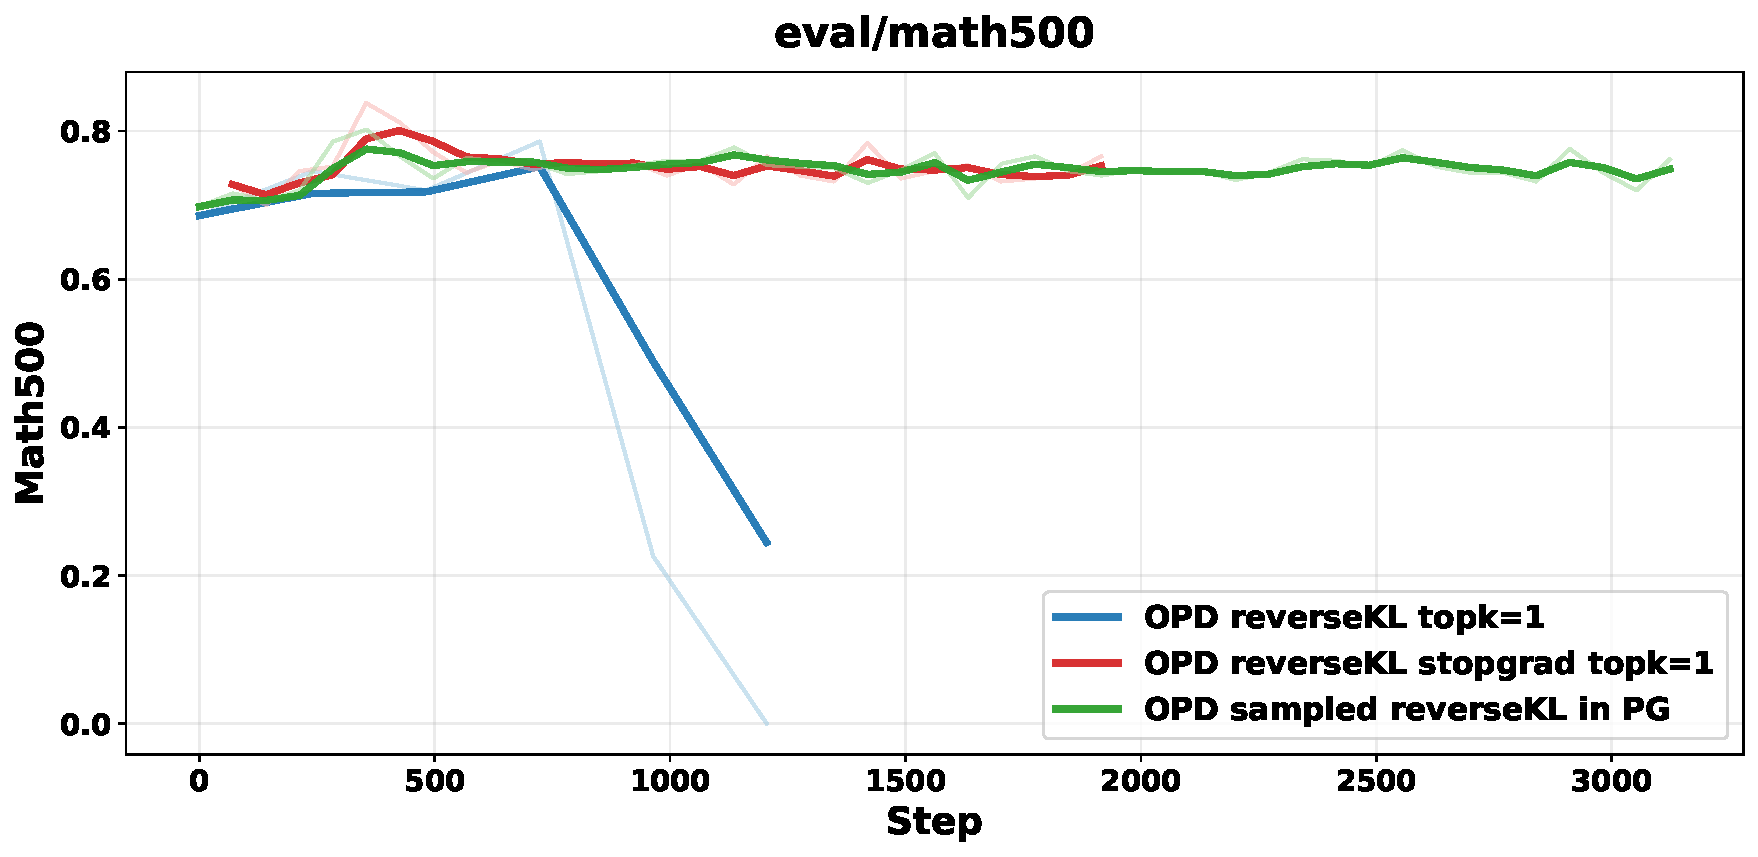
\includegraphics[width=\textwidth]{figures/PG_eval_math500.pdf}
        \label{fig:4b_char}
    \end{subfigure}
    \hfill
    % \begin{subfigure}[t]{0.33\textwidth}
    %     \centering
    %     \includegraphics[width=\textwidth]{figures/PG_repeat_ratio.pdf}
    %     \label{fig:4b_emo}
    % \end{subfigure}
    % \vspace{0.5em}
    \begin{subfigure}[t]{0.32\textwidth}
        \centering
        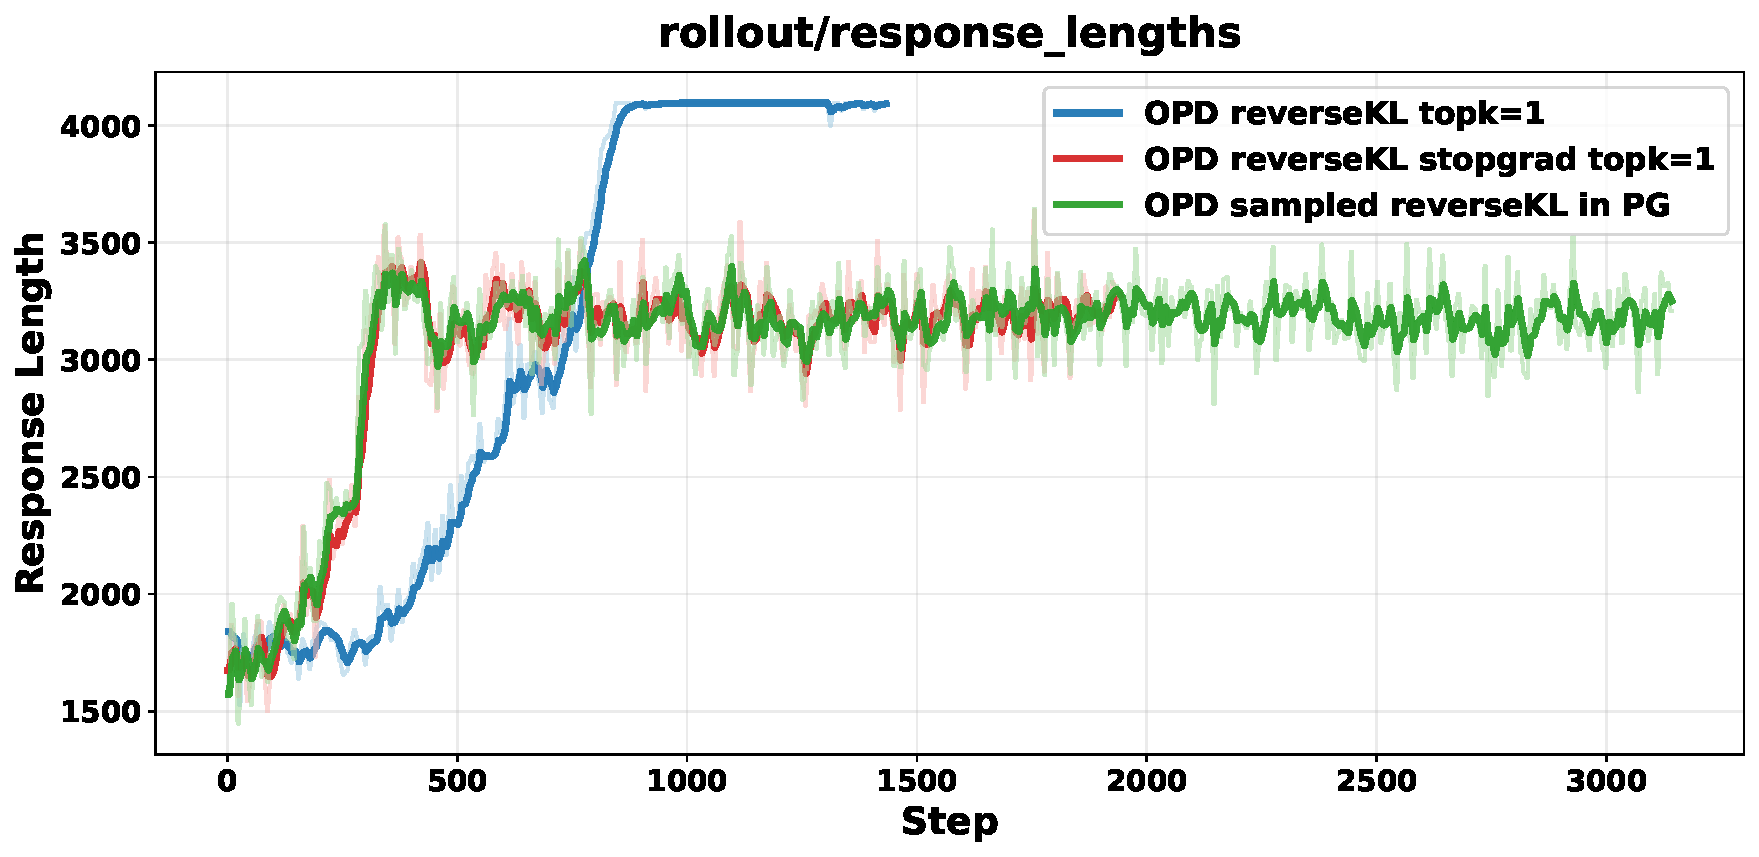
\includegraphics[width=\textwidth]{figures/PG_response_lengths.pdf}
        \label{fig:8b_char}
    \end{subfigure}
    \hfill
    \begin{subfigure}[t]{0.33\textwidth}
        \centering
        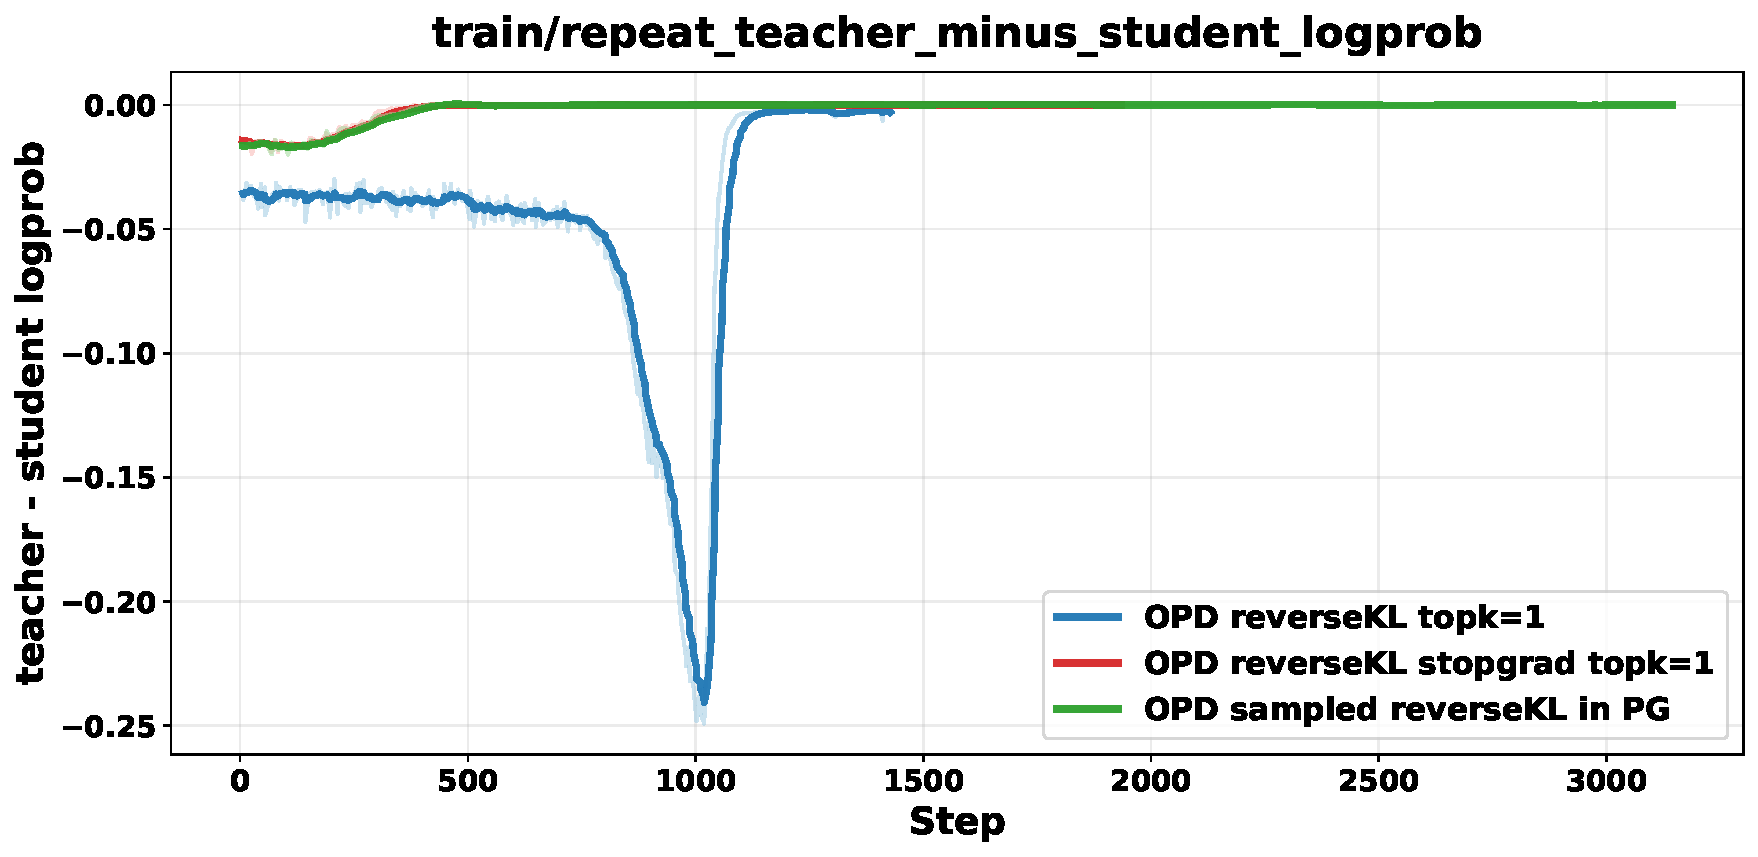
\includegraphics[width=\textwidth]{figures/PG_teacherstudent_repeat_logprob.pdf}
        \label{fig:8b_emo}
    \end{subfigure}
    \vspace{-2mm}
    \caption{Whether to put the distillation loss in policy gradient? sampled token KL in policy gradient is stable, while putting sampled token KL as a single loss (TopK=1) leads to model collapse. Teacher: Qwen3-1.7B-GRPO, Student: Qwen3-1.7B, dataset: DAPO}
    \label{fig:policygradexp}
\end{figure}


% \paragraph{Solution: Stop-Gradient Advantage Weighting.}

To mitigate the pathology of TopK reverse KL, we replace exact TopK reverse-KL with a stop-gradient version. Specifically, instead of differentiating through both \(\pi_S\) and \(\log \pi_S\), we stop gradients of the log-probability term. The resulting objective is
\begin{equation}
\mathcal L_{\mathrm{SG\text{-}Top}K}(t)
=
-\sum_{v\in S_K(y_{<t})} \pi_S(v\mid x,y_{<t})\, [\log \pi_T(v\mid x,y_{<t},I)-\operatorname{\textbf{stopgrad}}\!\bigl(\log \pi_S(v\mid x,y_{<t})\bigr)\bigr],
\label{eq:topksgKL}
\end{equation}
with gradient $\nabla_\theta \mathcal L_{\mathrm{SG\text{-}Top}K}(t)$:
\begin{equation}
-\sum_{v\in S_K(y_{<t})}
\pi_S(v\mid x,y_{<t})\, [\log \pi_T(v\mid x,y_{<t},I)-\!\log \pi_S(v\mid x,y_{<t})\bigr]\,\nabla_\theta \log \pi_S(v\mid x,y_{<t}).
\end{equation}
Although this objective is not the exact gradient of reverse KL, it is better aligned with the policy-gradient view of on-policy distillation, where the weighting term should act as an advantage rather than a differentiable part of the loss.



By contrast, this issue is much less severe for two alternative formulations. The first is the TopK reverse KL with renormalization. Let
\begin{equation}
\bar \pi_S
=
\frac{\pi_S(v\mid x,y{<t})}
{\sum_{u\in S_K(y{<t})} \pi_S(u\mid x,y{<t})},
\bar \pi_T
=
\frac{\pi_T(v\mid x,y{<t},I)}
{\sum_{u\in S_K(y{<t})} \pi_T(u\mid x,y{<t},I)}, 
v\in S_K(x,y{<t}).
\end{equation}
The renormalized TopK reverse KL is
\begin{equation}
\mathcal L_{\mathrm{Renorm}\text{-}\mathrm{Top}\text{-}K\text{-}\mathrm{RKL}}(t)
=
\sum_{v\in S_K(y{<t})}
\bar\pi_S(v\mid x,y{<t})
\log
\frac{\bar\pi_S(v\mid x,y{<t})}
{\bar\pi_T(v\mid x,y{<t},I)} .
\label{eq:renormtopkKL}
\end{equation}
Since distributions are normalized within the TopK set, the
constant $+1$ term cancels:
\begin{equation}
\sum_{v\in S_K(y_{<t})}
\bar\pi_S(v\mid x,y_{<t})
\nabla_\theta \log \bar\pi_S(v\mid x,y_{<t})
=
\nabla_\theta
\sum_{v\in S_K(y_{<t})}
\bar\pi_S(v\mid x,y_{<t})
=0.
\end{equation}
The gradient does not contain the $+1$ that causes the
unnormalized TopK reverse-KL bias in paragraph~\ref{curse_topk}. However, it only matches the relative probabilities
inside the selected TopK set and ignores the probability mass assigned
to that set. As a result, it mitigates the local gradient bias but no longer
faithfully approximates the full-vocabulary reverse KL.


A second alternative is to move the sampled-token signal into the policy-gradient (Equation\ref{eq:policygrad_sampledtoken}). This formulation also avoids the TopK reverse-KL issue. The drawback is that this objective uses only the sampled token \(y_t\). It therefore captures sparse teacher signal rather than the teacher vocabulary distribution.


\textbf{Another important design choice is the TopK truncation}. Ideally, we would like to query the teacher on the student's per-position TopK set $S_{\mathrm{stu},K}(y_{<t})$, or vice versa. 
However, this is not directly supported when using SGLang as inference engine (details in appendix \ref{topkchallenge}). 

Instead, we must take the union of all per-position TopK sets
$
U=\bigcup_{t=1}^T S_{\mathrm{stu},K}(y_{<t}),
$
and query this same global set at every position. If the response length is $T$, the ideal cost is $T\times K$, but the actual queried tensor becomes $T\times |U|$. 
In the worst case, the TopK sets at different positions are disjoint, so
$|U|=\min(|\mathcal V|,TK)$,
which increases memory by a factor of $\frac{\min(|\mathcal V|,TK)}{K}$. As a simple fix, we backpropagate only through tokens that appear in both models' TopK sets:
\begin{equation}
S_{K}(y_{<t}) = S_{\mathrm{tea},K}(y_{<t})\cap S_{\mathrm{stu},K}(y_{<t}) 
\end{equation}
Interestingly, prior work~\cite{li2026rethinkingonpolicydistillationlarge} finds that the teacher-student TopK intersection performs comparably to the student TopK, suggesting that our design does not degrade training effectiveness.



We compare three TopK objectives with $K=5$ in
Figure~\ref{fig:top5exp}: unnormalized reverse KL
(Equation~\ref{eq:topkrevKL}), its stop-gradient version
(Equation~\ref{eq:topksgKL}), and its renormalized version
(Equation~\ref{eq:renormtopkKL}). The unnormalized objective collapses during
training, whereas both modifications achieve comparable stable performance. We further test the formulation that places the distillation
signal within the policy gradient
(Equation~\ref{eq:policygrad_sampledtoken}). As shown in
Figure~\ref{fig:policygradexp}, it performs similarly to Top1 reverse KL with
stop-gradient, while the unmodified Top1 reverse KL still collapses. These
results suggest that correcting the biased reverse-KL gradient, through
stop-gradient, renormalization, or a policy-gradient formulation, is essential
for stable distillation.


% \subsection{SFT Stabilization}
% \siqi{for student}

% SFT can serve as both initialization and regularization for OPD. By pre-training the student on high-quality demonstrations, SFT provides a strong initialization that reduces the risk of early-stage collapse during on-policy distillation. It can also be combined with OPD as a regularization term, preventing the model from deviating too far from the SFT distribution and maintaining stable token-level supervision. This approach is particularly useful when the teacher-student distribution mismatch is large, or when the training data contains high variance in quality.


\subsection{Enhance teacher with RLVR.}

\begin{figure}[t]
    \centering
    \hfill
    \begin{subfigure}[t]{0.3\textwidth}
        \centering
        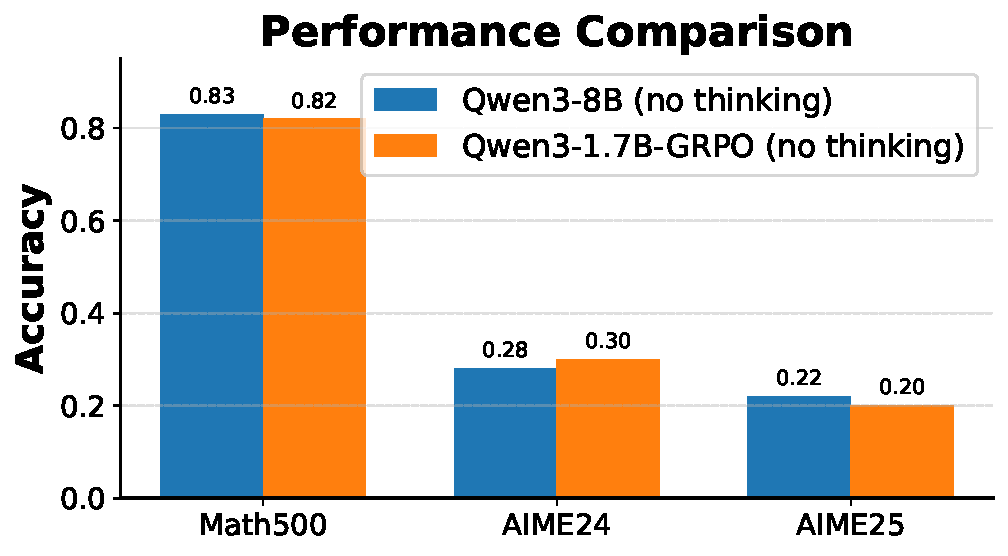
\includegraphics[width=\textwidth]{figures/qwen3_benchmark_comparison.pdf}
        \label{fig:second}
    \end{subfigure}
    \begin{subfigure}[t]{0.3\textwidth}
        \centering
        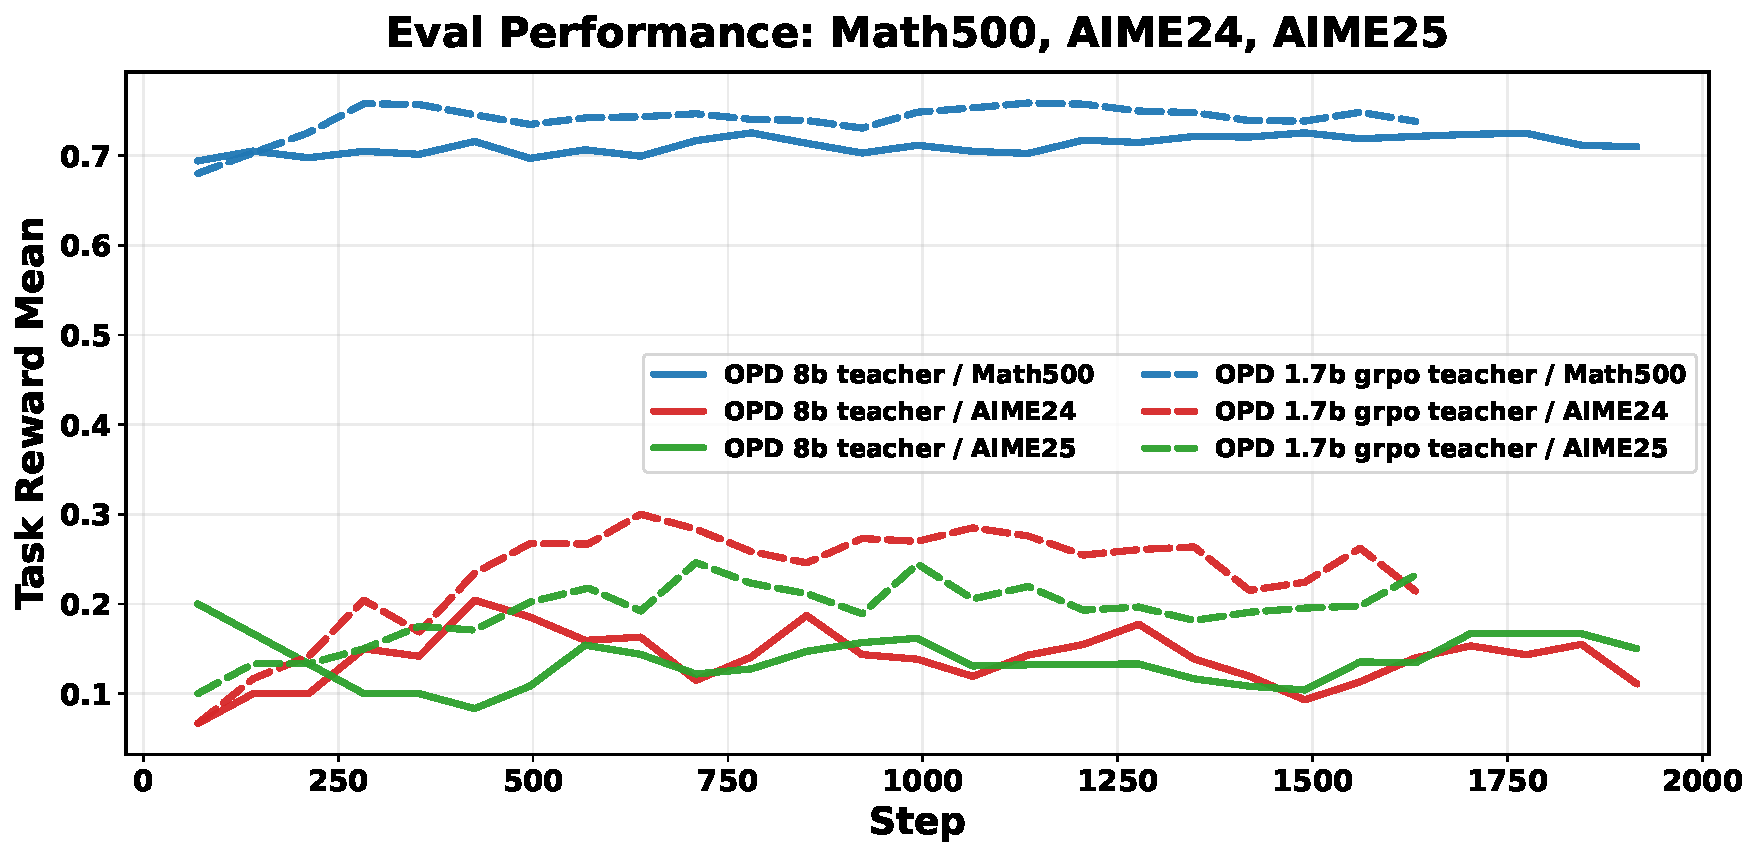
\includegraphics[width=\textwidth]{figures/1math500_aime24_aime25_eval.pdf}
        \label{fig:first}
    \end{subfigure}
    \hfill
    \begin{subfigure}[t]{0.3\textwidth}
        \centering
        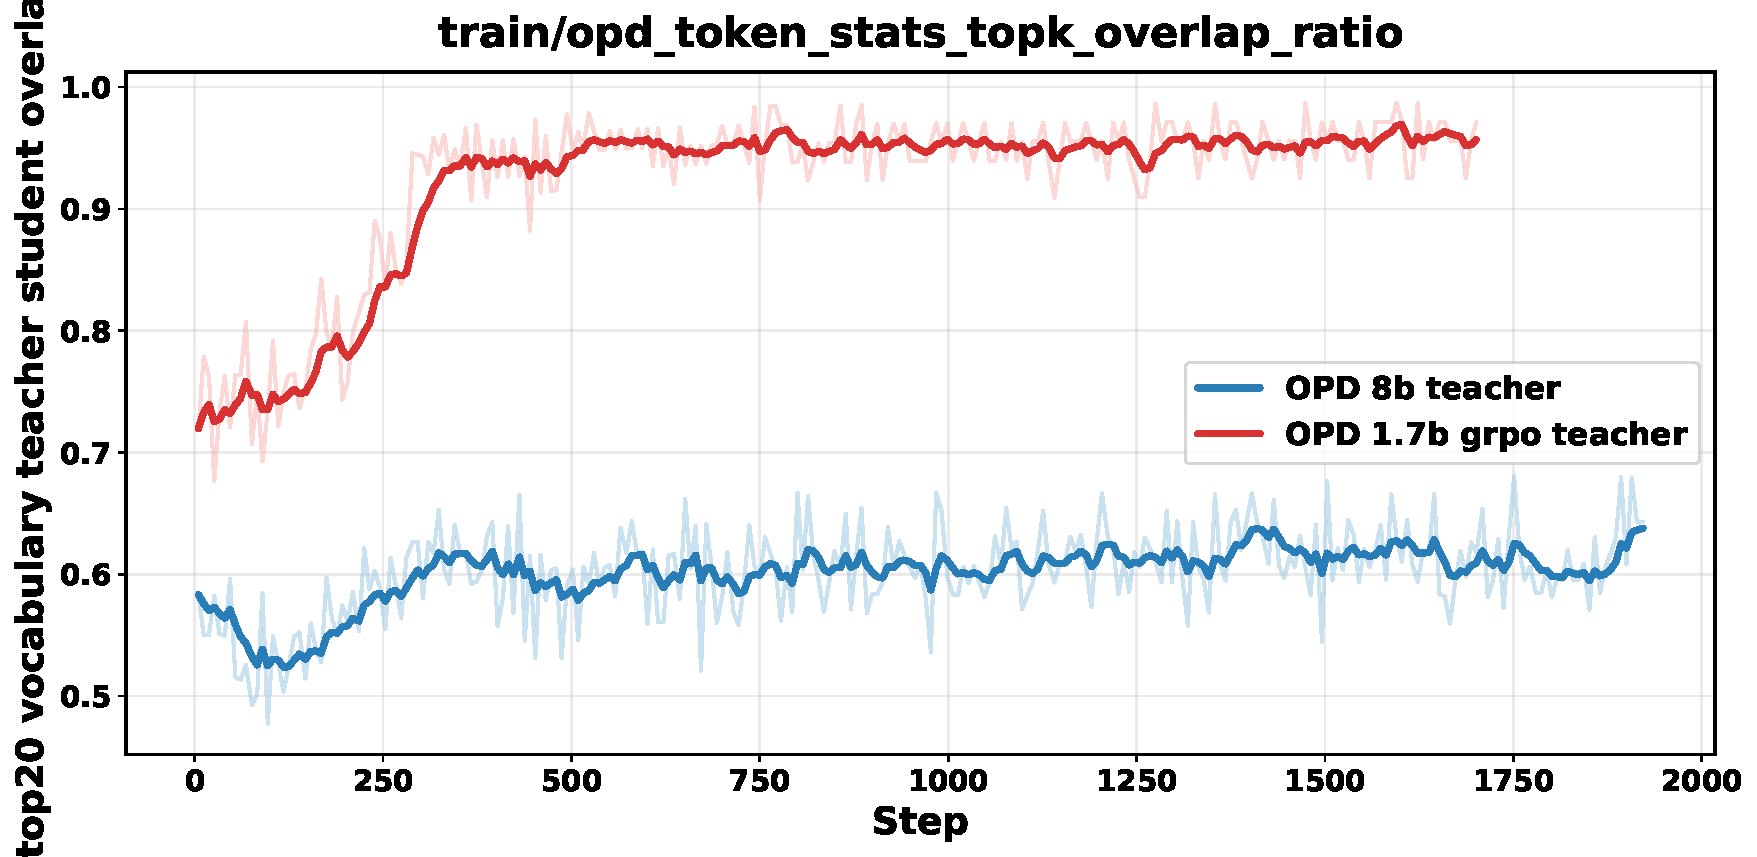
\includegraphics[width=\textwidth]{figures/1overlap_ratio_1.pdf}
        \label{fig:second}
    \end{subfigure}
    
    \vspace{-3mm}
    \caption{dataset: OpenThoughts. \textbf{Left}: Qwen3-8B and Qwen3-1.7B-GRPO have similar math reasoning performance. \textbf{Middle}: In OPD, Qwen3-1.7B-GRPO is a more effective teacher. \textbf{Right}: Qwen3-1.7B-GRPO's Top20 vocabulary distribution is more aligned with the Qwen3-1.7B student.}
    \label{fig:opsdrlvr}
\end{figure}


% \paragraph{RLVR-trained teachers mitigate distribution mismatch.}
One effective way to improve OPD is to adapt the teacher on the training
distribution before distillation. RLVR improves the teacher's task
performance on the training set and can make the teacher's
output distribution closer to that of the student. This reduces the
teacher-student distribution mismatch and makes token-level distillation signals
more locally compatible with the student's on-policy prefixes.

We evaluate this strategy in Figure\ref{fig:opsdrlvr}. We first train a Qwen3-1.7B model with
DAPO \cite{yu2025dapoopensourcellmreinforcement} for 200 steps, obtaining a RL-adapted teacher denoted
Qwen3-1.7B-GRPO. Qwen3-1.7B-GRPO achieves performance on
Math500, AIME24, and AIME25 that is comparable to Qwen3-8B. We then use either
Qwen3-1.7B-GRPO or Qwen3-8B as the teacher to distill a Qwen3-1.7B student on the
OpenThoughts \cite{guha2025openthoughtsdatarecipesreasoning} dataset. 

Although the two teachers have similar reasoning performance, distillation from Qwen3-1.7B-GRPO significantly outperforms
distillation from Qwen3-8B, suggesting that teacher accuracy alone is not
sufficient to predict OPD effectiveness. A teacher closer to the student distribution can provide stronger supervision, even if
it does not have stronger benchmark accuracy.
% More broadly, this suggests a more effective alternative to
% PI-based OP(S)D for math reasoning: first improve the model with RLVR,
% then distill from the RLVR-adapted checkpoint. 
Compared with using PI during distillation (Figures \ref{fig:2opsdfails} and \ref{fig:9OPDPI}), this pipeline
provides a stronger teacher and serves as an effective alternative to PI-based OP(S)D.


\subsection{Stabilize Student with SFT.}


\begin{figure}[t]
    \centering
    \begin{subfigure}[t]{\textwidth}
        \centering
        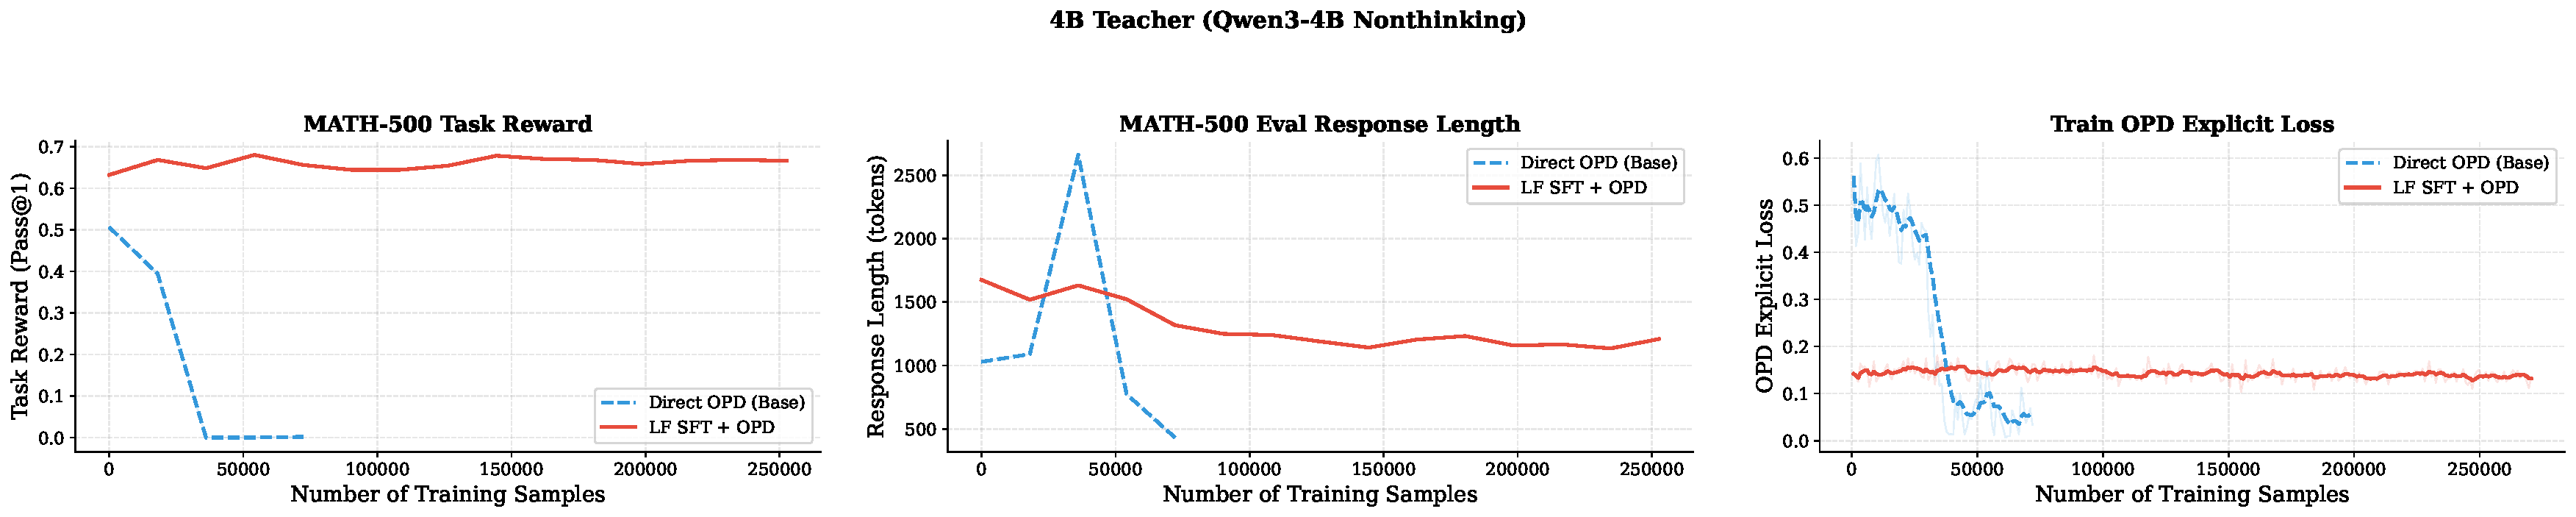
\includegraphics[
            width=\linewidth,
            trim=0 0 0 10mm,
            clip
        ]{figures/sft_opd_4b_teacher_combined.pdf}
        % \caption*{\small Qwen3-4B (nonthinking) teacher $\to$ Qwen3-1.7B-Base student.}
        \label{fig:sft_opd_4b}
    \end{subfigure}
    % \vspace{-4mm}
    % \begin{subfigure}[t]{0.9\textwidth}
    %     \centering
    %     \includegraphics[
    %         width=\linewidth,
    %         trim=0 0 0 10mm,
    %         clip
    %     ]{figures/sft_opd_7bmath_teacher_combined.pdf}
    %     \caption*{\small Qwen2.5-Math-7B-Instruct teacher $\to$ Qwen2.5-1.5B student.}
    %     \label{fig:sft_opd_7bmath}
    % \end{subfigure}
    \vspace{-3mm}
    \caption{
        Qwen3-4B teacher, Qwen3-1.7B-Base student, OpenThoughts. \textbf{Direct OPD} uses the student without SFT warm-up;
        \textbf{SFT + OPD} fine-tunes on teacher-generated traces before OPD.
    }
    \label{fig:sft_opd}
\end{figure}






Prior work has used supervised data to stabilize OPD. For example, Luo et al.~\cite{luo2026demystifying} combine OPD with SFT on gold answers to mitigate length inflation, while Li et al.~\cite{li2026rethinkingonpolicydistillationlarge} fine-tune the student on teacher-generated traces to reduce the teacher-student distribution mismatch. In the Qwen3-4B $\rightarrow$ Qwen3-1.7B-Base setting, we observe a distinct instability source: the 1.7B student initially produces garbled, nonsensical outputs (non-English Unicode) in some questions. Unlike ordinary incorrect reasoning, these outputs contain degenerate sequences with little semantic structure. In this case, teacher is unlikely to provide a meaningful signal, making Direct OPD unstable. As shown in Figure~\ref{fig:sft_opd}, teacher-trace SFT regularizes the student's output space, stabilizes response length, and allows subsequent OPD to improve accuracy. These results suggest that SFT helps OPD by keeping on-policy samples in well-formed regions where teacher feedback remains effective. Experiment details are in Appendix~\ref{app:experiment_setup_6.3}.